\documentclass{beamer}

\usepackage[utf8]{inputenc}
\usepackage[english]{babel}
\usepackage{etex}
\usepackage{graphicx}
\usepackage{color}
\usepackage{hyperref}
\usepackage{verbatim}
\usepackage{url}
\usepackage{moreverb}
\usepackage{fancyvrb}
\usepackage{minted}
\usepackage{natbib}
\usepackage{eulervm}
\usepackage{auto-pst-pdf}
\usepackage{pst-plot}
\usepackage{amssymb}
\usepackage{pifont}

% Checked marks
\newcommand{\cmark}{\ding{51}}%
\newcommand{\xmark}{\ding{55}}%

% Colors
\newrgbcolor{mygreen}{.00 .5 .00}
\newcommand{\X}[1]{\textcolor{blue}{#1}}
\newcommand{\y}[1]{\textcolor{red}{#1}}
\newcommand{\model}[1]{\textcolor{mygreen}{#1}}
\newcommand{\loss}[1]{\textcolor{lightblue}{#1}}

% Beamer layout
\hypersetup{colorlinks=true, linkcolor=black, urlcolor=blue}
\usetheme{boxes}
\beamertemplatenavigationsymbolsempty
\setbeamertemplate{sections/subsections in toc}[circle]
\setbeamertemplate{footline}[frame number]
\setbeamertemplate{itemize items}[circle]
\setbeamertemplate{itemize subitem}[square]

% Front slide
\title{{\bf Tree models with Scikit-Learn}\\
Great learners with little assumptions}
\author{
Material: \url{https://github.com/glouppe/talk-pydata2015}\\
\vspace{1cm}
Gilles Louppe (\href{https://twitter.com/glouppe}{@glouppe})\\
{\it CERN}
}
\date{PyData, April 3, 2015}

% Argmax
\DeclareMathOperator*{\argmax}{arg\,max}

\begin{document}

\begin{frame}
\titlepage
\end{frame}


% Random things to talk about:
% - class_weights
% - oob samples
% - n_jobs


% Outline =====================================================================

\begin{frame}
  \frametitle{Outline}
  %\tableofcontents
  \setbeamertemplate{enumerate items}[circle]
  \begin{enumerate}
  \item Motivation

  \vspace{0.5cm}

  \item Growing decision trees

  \vspace{0.5cm}

  \item Random forests

    \vspace{0.5cm}

  \item Boosting

  \vspace{0.5cm}

  \item Reading tree leaves

  \vspace{0.5cm}

  \item Summary
  \end{enumerate}
\end{frame}


% Motivation ==================================================================

\section{Motivation}

\begin{frame}
    \frametitle{Motivation}
    \begin{figure}
    \vspace{-0.5cm}
    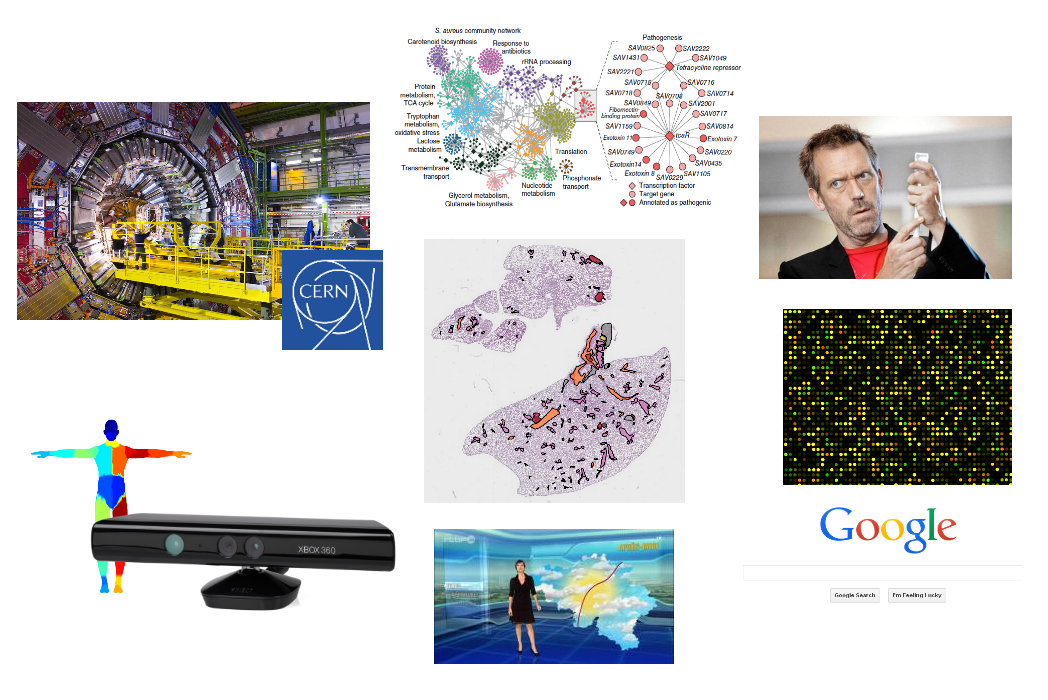
\includegraphics[scale=0.4]{./figures/motivation.png}
    \end{figure}
\end{frame}

\begin{frame}
    \frametitle{Running example}

    \begin{columns}
    \begin{column}{0.5\textwidth}

    \begin{center}
    From {\bf \X{physicochemical properties}} (alcohol, acidity, sulphates, ...),

    \vspace{1cm}
    learn a {\bf \model{model}}
    \vspace{1cm}

    to predict {\bf \y{wine taste preferences}}.

    \end{center}

    \end{column}
    \begin{column}{0.5\textwidth}
      \begin{figure}
      \vspace{-0.5cm}
      
\includegraphics[scale=0.6]{./figures/wine.jpg}
      \end{figure}
    \end{column}
    \end{columns}
\end{frame}


% Growing decision trees ======================================================

\AtBeginSection[]
{
\begin{frame}
  \frametitle{Outline}
  \tableofcontents[currentsection]
  % Die Option [pausesections]
\end{frame}
}

\section{Growing decision trees}

\begin{frame}[fragile]
    \frametitle{Supervised learning}

    \begin{itemize}
    \item Data comes as a finite learning set ${\cal L} = \texttt{(\X{X}, \y{y})}$ where
        \begin{itemize}
            \item \X{Input samples} are given as an array of shape \texttt{(n\_samples, n\_features)}\\
            \vspace{0.25cm}
            E.g., feature values for the physicochemical properties:
\begin{verbatim}
X = [[  7.4    0.     ...   0.56   9.4    0.  ]
     [  7.8    0.     ...   0.68   9.8    0.  ]
                      ...
     [  7.8    0.04   ...   0.65   9.8    0.  ]]
\end{verbatim}
\vspace{0.25cm}

            \item \y{Output values} are given as an array of shape \texttt{(n\_samples,)}\\
            \vspace{0.25cm}
            E.g., wine taste preferences (from 0 to 10):
\begin{verbatim}
y = [5 5 5 ... 6 7 6]
\end{verbatim}
        \end{itemize}

    \vspace{0.25cm}

    \item The goal is to build an estimator $\model{\varphi_{\cal L}}: \X{{\cal X}} \mapsto \y{{\cal Y}}$ minimizing
    $$
    Err(\model{\varphi_{\cal L}}) = \mathbb{E}_{\X{X},\y{Y}}\{ L(\y{Y}, \model{\varphi_{\cal L}}\texttt{.predict(}\X{X}\texttt{)}) \}.
    $$
    \end{itemize}
\end{frame}

\begin{frame}
  \frametitle{Divide and conquer}
\end{frame}

\begin{frame}
  \frametitle{Decision trees framework}
  % framework impurity / simple model at leaves => mention density estimation, classifi and regression
\end{frame}

\begin{frame}
  \frametitle{Strengths and weaknesses}
  % use a continued table from slide to sldie
\end{frame}


% Forests and boosting ========================================================

\section{Random Forests}

\begin{frame}
  \frametitle{Bias-variance decomposition}
\end{frame}

\begin{frame}
  \frametitle{Random Forests}
\end{frame}

\begin{frame}
  \frametitle{Strengths and weaknesses}
\end{frame}


% Forests and boosting ========================================================

\section{Boosting}

\begin{frame}
  \frametitle{Gradient Boosted Regression Trees}
\end{frame}

\begin{frame}
  \frametitle{Strengths and weaknesses}
\end{frame}

% Framework (loss function, regularization, etc)


% Reading tree leaves =========================================================

\section{Reading tree leaves}

\begin{frame}
  \frametitle{Reading tree leaves}
  % Visualizing trees
\end{frame}

\begin{frame}
  \frametitle{Variable importances}
\end{frame}

\begin{frame}
  \frametitle{Partial dependence plots}
\end{frame}

\begin{frame}
  \frametitle{Outlier detection}
\end{frame}

\begin{frame}
  \frametitle{Embedding}
\end{frame}



% Summary =================================================================

% strong points and weaknesses
% going further


\section{Summary}

\begin{frame}
  \frametitle{Summary}
\end{frame}

\begin{frame}
\begin{center}
{\Huge  Questions?}
\end{center}
\end{frame}

\end{document}
